\section{Results and discussion}
% Define a custom command to create sections with shared structure

As explained in \ref{sec:methodo}, the first objective is to effectively post-process a single NWP forecast model, by benchmarking the models altogether. 

The following step will be to look at the results in the details to prove the true effectiveness of the post-processing.
\subsection{Post-processing of a single forecasting NWP model}
\subsubsection{Study of the models altogether} 
\paragraph{MAE}
\begin{figure}[htb!]
    \centering
    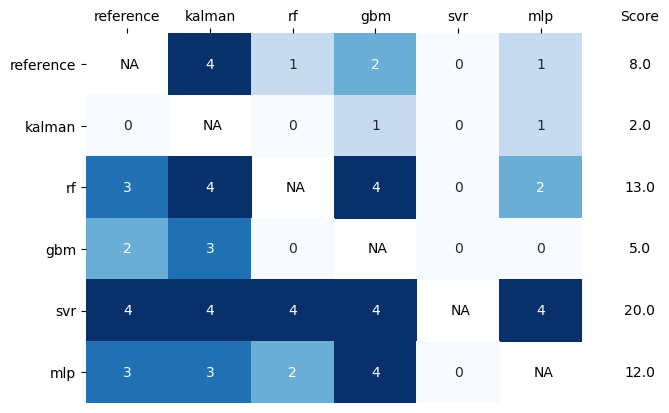
\includegraphics[width=\columnwidth]{figures/first_study/significance_matrix_mae.png}
\caption{Significance matrix for MAE. The value $V_{(i,j)}$ of the $(i,j)$ cell indicates how often the model of line i performs better than the one of column j, across the 
4 sites. For example, the MAE of the MLP model post-processed data is 3 times lower than the MAE of the reference model, and for 1 site (4 - 3 = 1), it is higher.}
\end{figure}

\begin{figure}[htb!]
    \centering
    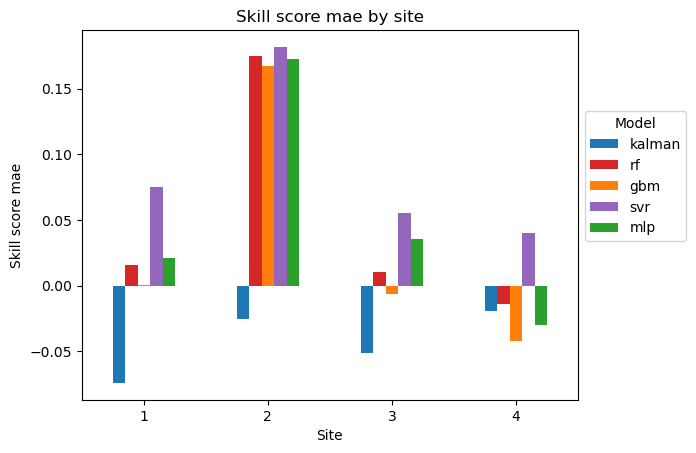
\includegraphics[width=\columnwidth]{figures/first_study/ss_mae.png}
    \caption{MAE skill score plot across the 4 sites.}
\end{figure}
\paragraph{RMSE}

\begin{figure}[htb!]
    \centering
    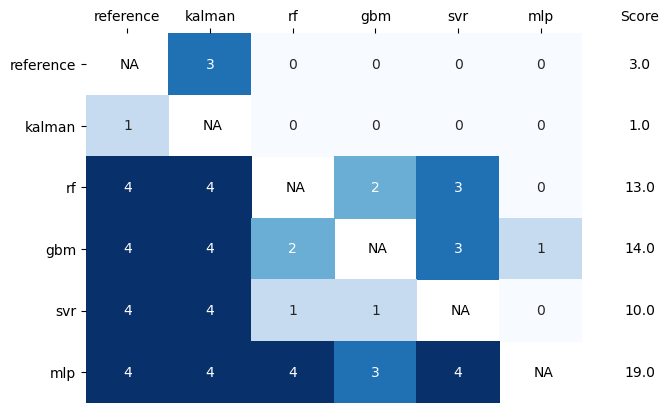
\includegraphics[width=\columnwidth]{figures/first_study/significance_matrix_rmse.png}
\caption{Significance matrix for RMSE. The value $V_{(i,j)}$ of the $(i,j)$ cell indicates how often the model of line i performs better than the one of column j, across the 
4 sites. For example, the RMSE of the MLP model post-processed data is 3 times lower than the RMSE of the reference model, and for 1 site (4 - 3 = 1), it is higher.}
\end{figure}

\begin{figure}[htb!]
    \centering
    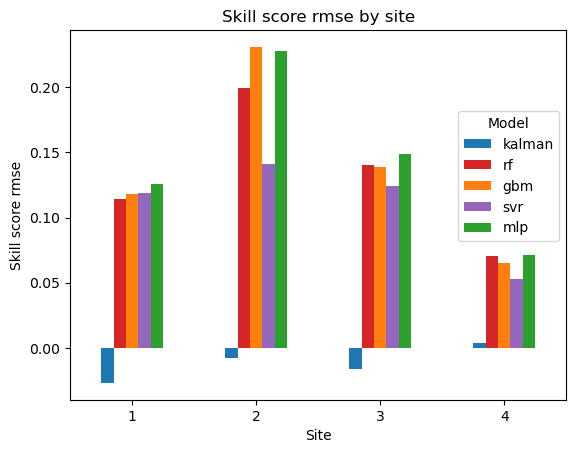
\includegraphics[width=0.75\columnwidth]{figures/first_study/ss_rmse.png}
    \caption{RMSE skill score plot across the 4 sites.}
\end{figure}

\subsubsection{Detailled study of the most performing model}
With the aim of clarity, only the plots of the single site 2 will be shown here.
The overall similarity of the results across the 4 sites also motivate this choice.

The ones of the other sites can be found in the appendix to fortify the belief in the analysis drawn for a single site.

\paragraph{MAE}
\begin{figure}[htb!]
    \centering
    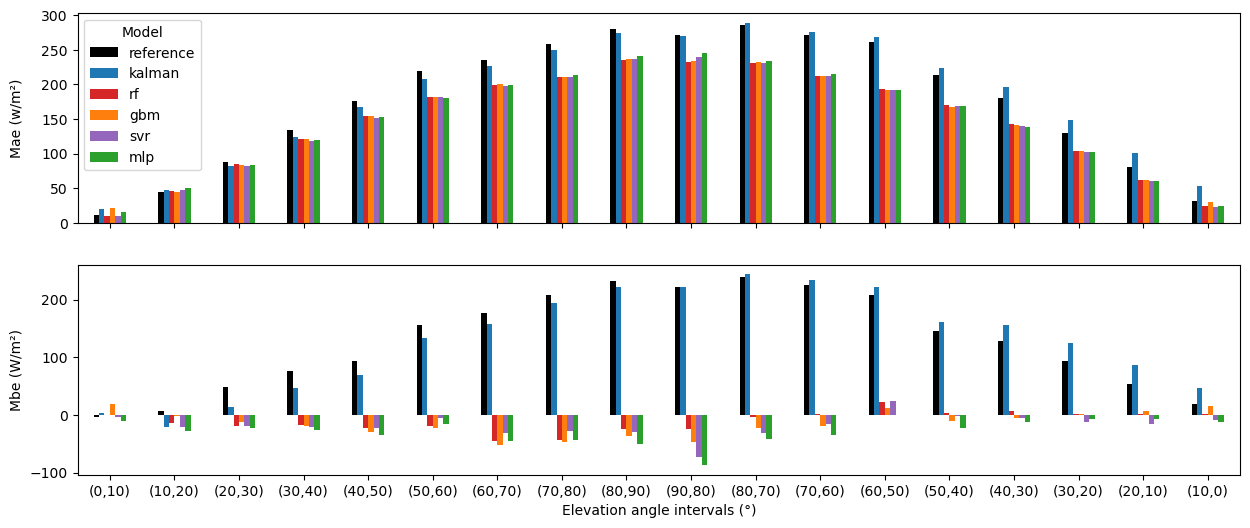
\includegraphics[width=\columnwidth]{figures/first_study/mae_mbe_site2.png}
\caption{MAE and MBE levels across all elevation angle intervals of a day, for site 2.}
\end{figure}

\begin{figure}[htb!]
    \centering
    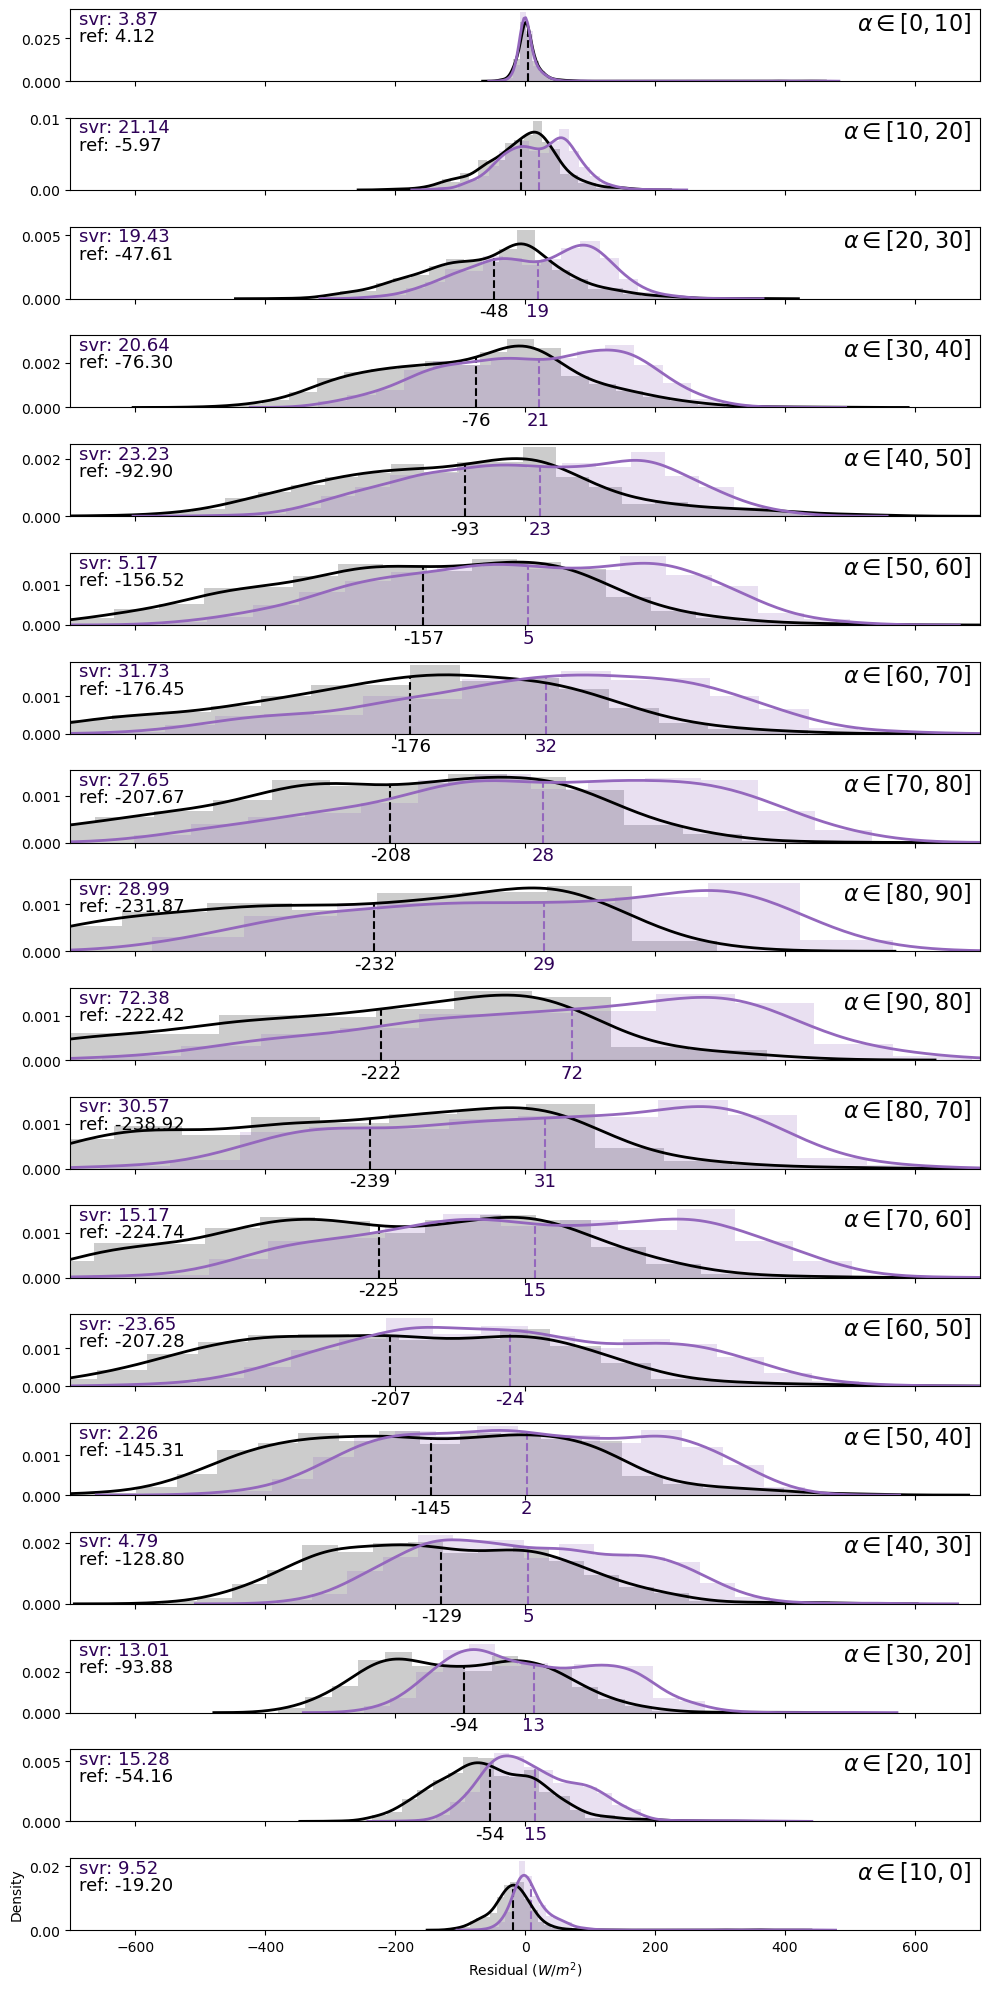
\includegraphics[width=\columnwidth]{figures/first_study/residual_errors_svr_site2_mae.png}
\caption{Residual error levels across all elevation angle intervals of a day, for a SVR model, for site 2.}
\end{figure}


\paragraph{RMSE}
\begin{figure}[htb!]
    \centering
    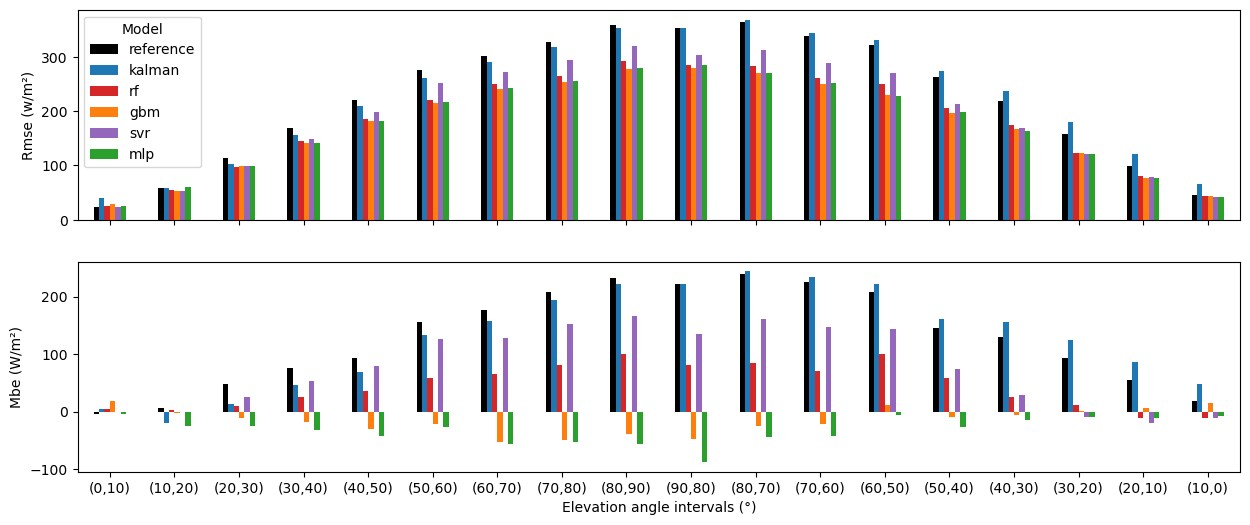
\includegraphics[width=\columnwidth]{figures/first_study/rmse_mbe_site2.png}
\caption{RMSE and MBE levels across all elevation angle intervals of a day, for site 2.}
\end{figure}

\begin{figure}[htb!]
    \centering
    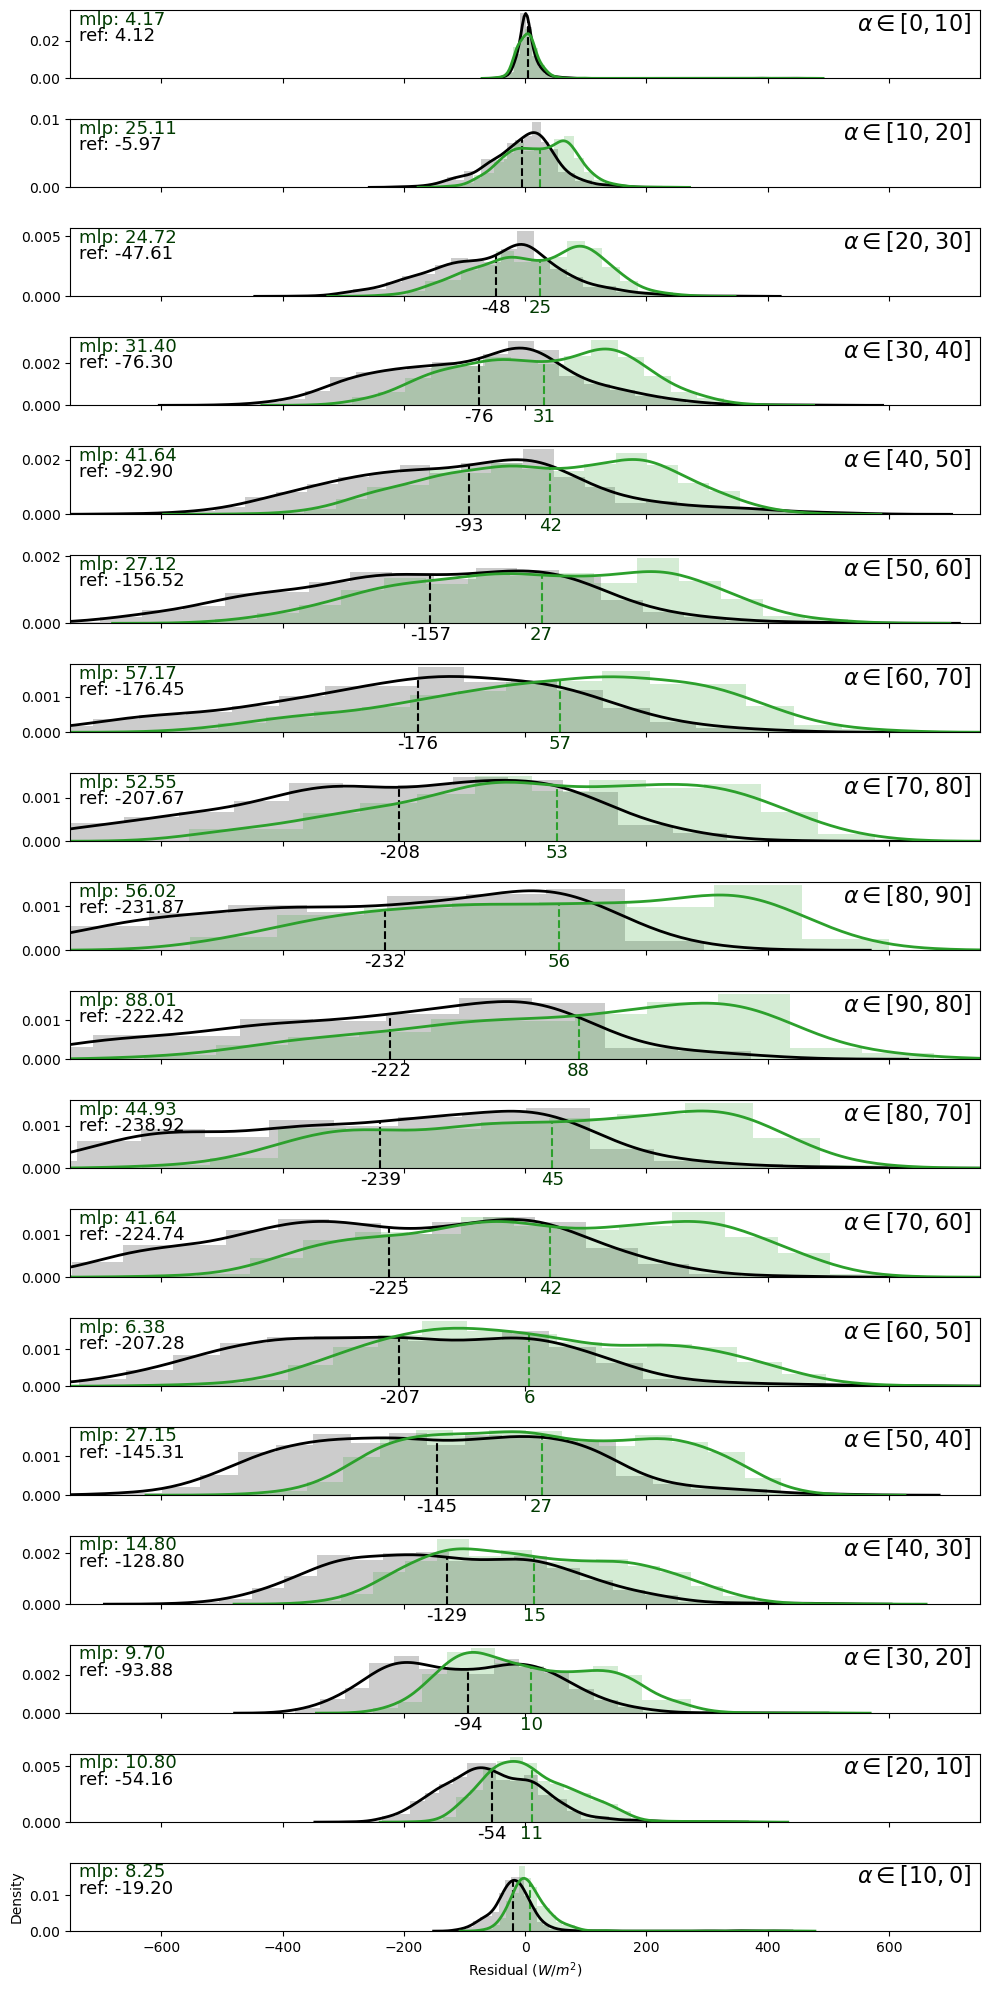
\includegraphics[width=\columnwidth]{figures/first_study/residual_errors_mlp_site2_rmse.png}
\caption{Residual error levels across all elevation angle intervals of a day, for a MLP model, for site 2.}
\end{figure}

\subsubsection{Sensitivity study}
It is also necessary to perform a sensitivity study of the parameters that are not tuned in our process. It is why the influence of the choices of predictors, of learning periods, of learning window type (fixed or sliding).
and of forecasting model are successively performed. 

With the aim of clarity, the results will be here presented with the MAE optimisation, but the results of the RMSE optimisation lead the same conclusions, and can also
be found in the appendix.

\paragraph{Influence of the choice of the predictors}
\begin{table}[htb!]
\begin{center}
\begin{tabular}{|l|llll|}
\toprule
{} &  0 &  1 &  2 &  3 \\
\midrule
$ghi_{GFS}$            &  X &  X &  X &  X \\
$temperature^{2m}_{GFS}$ &  X &  X &    &    \\
$\theta$             &  X &  X &  X &    \\
$\phi$            &  X &  X &  X &    \\
$ghi_{cs}$             &  X &    &  X &    \\
\bottomrule
\end{tabular}
\end{center}
\label{tab:pred_configs}
\caption{Description of the configurations of the sets of predictors.}
\end{table}

\begin{figure}[htb!]
    \centering
    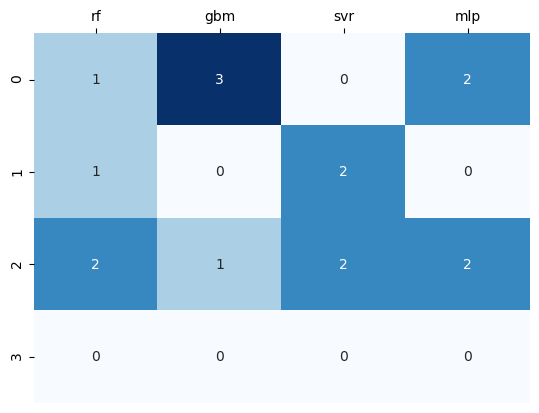
\includegraphics[width=\columnwidth]{figures/first_study/comp_predictors_mae.png}
\caption{Pairwise systematicity matrix for MAE. The value $V_{i,j}$ of the cell $(i,j)$ indicates how often the configuration of line i is the best one, across the 4 sites, for the model of column j. For example, the configuration 0 is the best one with a GBM post-processing for 3 sites, and the configuration 2 is the best one for 1 site.}
\end{figure}

\begin{figure}[htb!]
    \centering
    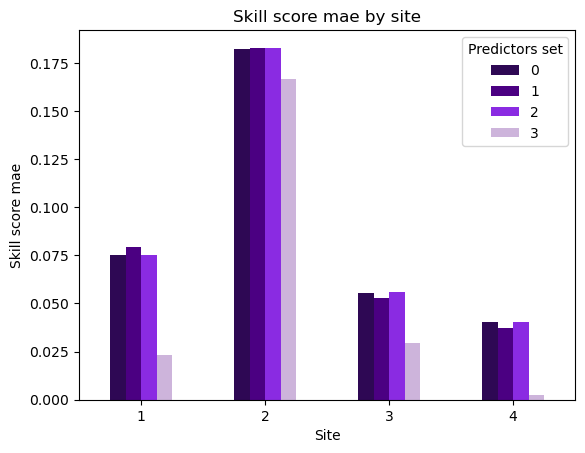
\includegraphics[width=\columnwidth]{figures/first_study/comp_predictors_mae_svr.png}
\caption{Comparison of the MAE skill scores of the different configurations.}
\end{figure}

\paragraph{Influence of the learning period}
\begin{figure}[htb!]
    \centering
    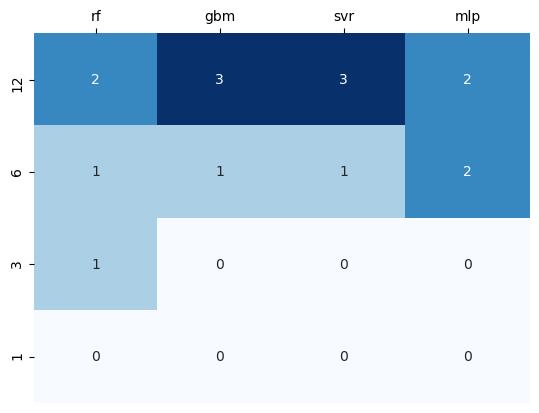
\includegraphics[width=\columnwidth]{figures/first_study/comp_learning_period_mae.png}
\caption{Pairwise systematicity matrix for MAE. The value $V_{i,j}$ of the cell $(i,j)$ indicates how often the learning period duration (in months) of line i performs the best, across the 4 sites, for the model of column j. For example, having a 12-months-long learning period is the best thing in 3 sites out of 4 with a SVR model, the last site performs better with a 6-month-long learning period.}
\end{figure}

\begin{figure}[htb!]
    \centering
    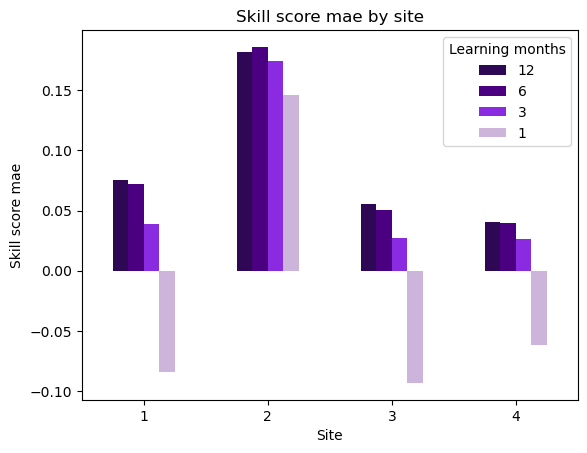
\includegraphics[width=\columnwidth]{figures/first_study/comp_learning_period_mae_svr.png}
\caption{Comparison of the MAE skill scores of the different learning period durations (in months).}
\end{figure}

\paragraph{Influence of the window of learning}

\begin{figure}[htb!]
    \centering
    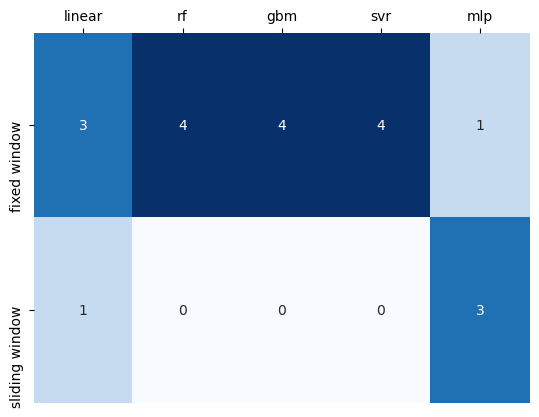
\includegraphics[width=\columnwidth]{figures/first_study/comp_window_mae.png}
\caption{Pairwise systematicity matrix concerning window type for MAE.}
\end{figure}

\begin{figure}[htb!]
    \centering
    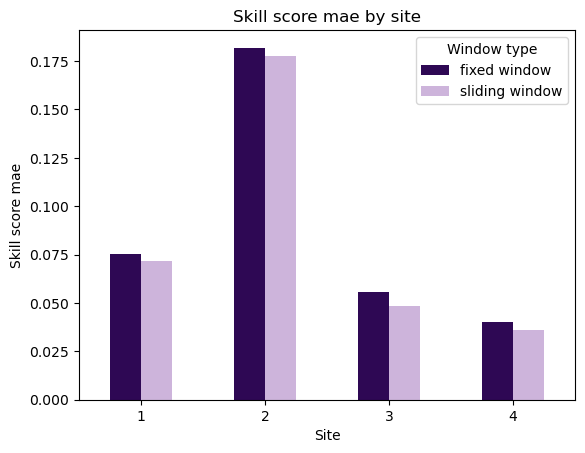
\includegraphics[width=\columnwidth]{figures/first_study/comp_window_mae_svr.png}
\caption{Comparison of the MAE skill scores for a SVR model.}
\end{figure}

\paragraph{Influence of the NWP forecasting model}

\begin{figure}[htb!]
    \centering
    \includesvg[width=\columnwidth]{figures/first_study/comp_for_models_mae.svg}
\caption{Comparison of the post-processing of four different NWP forecast models on MAE.}
\end{figure}
\subsection{Benchmarking the linear regression models}

\paragraph{MAE}
\begin{figure}[htb!]
    \centering
    \includesvg[width=\columnwidth]{figures/linear_study/mae_matrix.svg}
\caption{Significance matrix for MAE. Models at the top of the matrix are the most succesful ones, on the criterium of the sum of the values of each line. The value $V_{(i,j)}$ of the $(i,j)$ cell indicates how often the model of line i performs better than the one of column j, across the 
4 sites. For example, the MAE of the Lars model post-processed data is 1 times lower than the MAE of the Lasso model, and for 1 site (4 - 1 = 3), it is higher.}
\end{figure}

\begin{figure}[htb!]
    \centering
    \includesvg[width=\columnwidth]{figures/linear_study/mae_ss.svg}
\caption{MAE skill score plots of the best linear models.}
\end{figure}


\paragraph{RMSE}
\begin{figure}[htb!]
    \centering
    \includesvg[width=\columnwidth]{figures/linear_study/rmse_matrix.svg}
\caption{Significance matrix for RMSE. Models at the top of the matrix are the most succesful ones, on the criterium of the sum of the values of each line. The value $V_{(i,j)}$ of the $(i,j)$ cell indicates how often the model of line i performs better than the one of column j, across the 
4 sites. For example, the RMSE of the Lars model post-processed data is 1 times lower than the RMSE of the Lasso model, and for 1 site (4 - 1 = 3), it is higher.}
\end{figure}

\begin{figure}[htb!]
    \centering
    \includesvg[width=\columnwidth]{figures/linear_study/rmse_ss.svg}
\caption{RMSE skill score plots of the best linear models.}
\end{figure}
\subsection{Showcase of the hybrid model}
\subsubsection{Study on the four inital sites}
\begin{figure}[htb!]
    \centering
    \includesvg[width=\columnwidth]{figures/final_study/widen_time_window.svg}
\caption{Comparison of the two versions of LT CONT.}
\end{figure}
\paragraph{MAE}
\begin{figure}[htb!]
    \centering
    \includesvg[width=\columnwidth]{figures/final_study/ss_best_mae.svg}
\caption{MAE skill score plots of the relevant models, the reference being here the best NWP forecast (in practise, this means ECMWF).}
\end{figure}

\begin{figure}[htb!]
    \centering
    \includesvg[width=\columnwidth]{figures/final_study/evolution_plot_mae.svg}
\caption{MAE evolution of the relevant models.}
\end{figure}


\paragraph{RMSE}
\begin{figure}[htb!]
    \centering
    \includesvg[width=\columnwidth]{figures/final_study/ss_best_rmse.svg}
\caption{RMSE skill score plots of the relevant models, the reference being here the best NWP forecast (in practise, this means ECMWF).}
\end{figure}

\begin{figure}[htb!]
    \centering
    \includesvg[width=\columnwidth]{figures/final_study/evolution_plot_rmse.svg}
\caption{RMSE evolution of the relevant models.}
\end{figure}

\subsubsection{Study on the German sites}

\begin{figure}[htb!]
    \centering
    \includesvg[width=\columnwidth]{figures/german_sites.svg}
\caption{The 25 German sites used for validation.}

\end{figure}
\paragraph{MAE}
\begin{figure}[htb!]
    \centering
    \includesvg[width=\columnwidth]{figures/final_study/ss_heatmap_mae.svg}
\caption{MAE skill score heatmap of the validation sites.}
\end{figure}
\paragraph{RMSE}
\begin{figure}[htb!]
    \centering
    \includesvg[width=\columnwidth]{figures/final_study/ss_heatmap_rmse.svg}
\caption{RMSE skill score heatmap of the validation sites.}
\end{figure}


\begin{figure}[htb!]
    \centering
    \includesvg[width=\columnwidth]{figures/final_study/ss_heatmap_rmse_linear_4_sites.svg}
\caption{Global linear model verification on the 4 initial sites.}
\end{figure}